\chapter{Inpainting rapide d'images spatialement lisses}
\label{ch-chapter_3}
\dochaptoc
%
\section{Contexte des données EELS spatialement lisses}

Ce chapitre se focalise sur les images spatialement lisses, \ie{}, dont l'évolution spatiale est lente. En microscopie STEM-EELS, deux situations peuvent aboutir à ce type d'image : soit l'image est basse résolution, soit l'échantillon est amorphe ou mal orienté.

\subsection{Contexte des images basses résolution}\label{sec-donnees-sous-echantillonnees}


Les images basse résolution déjà présentées à la \cref{sec-prop-eels} sont acquises sur des échelles relativement grandes (typiquement \np[nm]{100}) afin de visualiser les structures présentes dans l'échantillon. 
%
Or, le nombre de pixels que l'on peut s'autoriser à échantillonner est limité afin d'empêcher une trop grande détérioration de l'échantillon. 
%
C'est pourquoi les images \gls{eels} acquises sur de telles échelles sont volontairement fortement sous-échantillonnées, elles ont généralement une résolution relativement faible comparée au pouvoir séparateur de l'instrument, \ie\ qu'un pixel d'une image basse résolution représente de nombreux atomes. 
%
Par exemple, l'image \gls{haadf} (acquise simultanément à l'image \gls{eels}) donnée sur la figure~\ref{fig-BR-haadf-b} a une taille de pixel de \np[nm]{2}, soit approximativement 20 colonnes atomiques, ou encore 2 fois (resp. 20 fois) le pouvoir de séparation du VG-HB501 (resp. du Nion UltraSTEM 200) dont dispose le \gls{lps}.
%
Il en résulte que, dans le cas d'une acquisition complète du spectre-image, un problème de super-résolution\footnote{La super-résolution ne fait pas référence ici aux techniques de microscopie par émission stimulée mises au point pour dépasser la limite de résolution imposée par la diffraction. Il s'agit ici d'un problème en traitement de l'image permettant d'augmenter la résolution, \ie{} le nombre de pixels par unité de longueur.} (couplé à du débruitage) peut être posé afin de restituer une image dont la résolution est identique au pouvoir séparateur de l'appareil. \`A cela vient s'ajouter le problème d'inpainting formulé dans la section précédente lorsque l'acquisition est incomplète. Dans le cadre de cette étude, le problème de super-résolution ne sera pas considéré et les résolutions des images acquise et reconstruite seront les mêmes.

En ce qui concerne les images basse résolution, les distorsions associées à l'acquisition, en particulier la dérive de l'échantillon, sont supposées être négligeables par rapport à la taille du pixel (ce qui n'est pas vrai pour les données haute résolution comme nous le verrons au \cref{ch-chapter_4}). Et puisque la résolution de l'image est faible, celle-ci est généralement spatialement lisse et rentre dans le cadre de ce chapitre.

Il faut noter que l'acquisition d'une image \gls{haadf} requiert un temps d'exposition de l'ordre le la microseconde, contre un temps de l'ordre de la milliseconde pour l'acquisition \gls{eels}, ce qui permet de visiter davantage de pixels à dose totale fixée. En général, cela permet de visualiser les structures suivant un angle de vue plus large et de localiser la zone d'intérêt, comme le montre la \cref{fig-BR-haadf-a}. A contrario, l'acquisition \gls{eels} (ainsi que l'image \gls{haadf} acquise de manière simultanée) est très localisée et sa taille est très réduite, comme le montre la \cref{fig-BR-haadf-b}.

\begin{figure}[t]
    \centering
    \subfigure[\label{fig-BR-haadf-a}]%
    {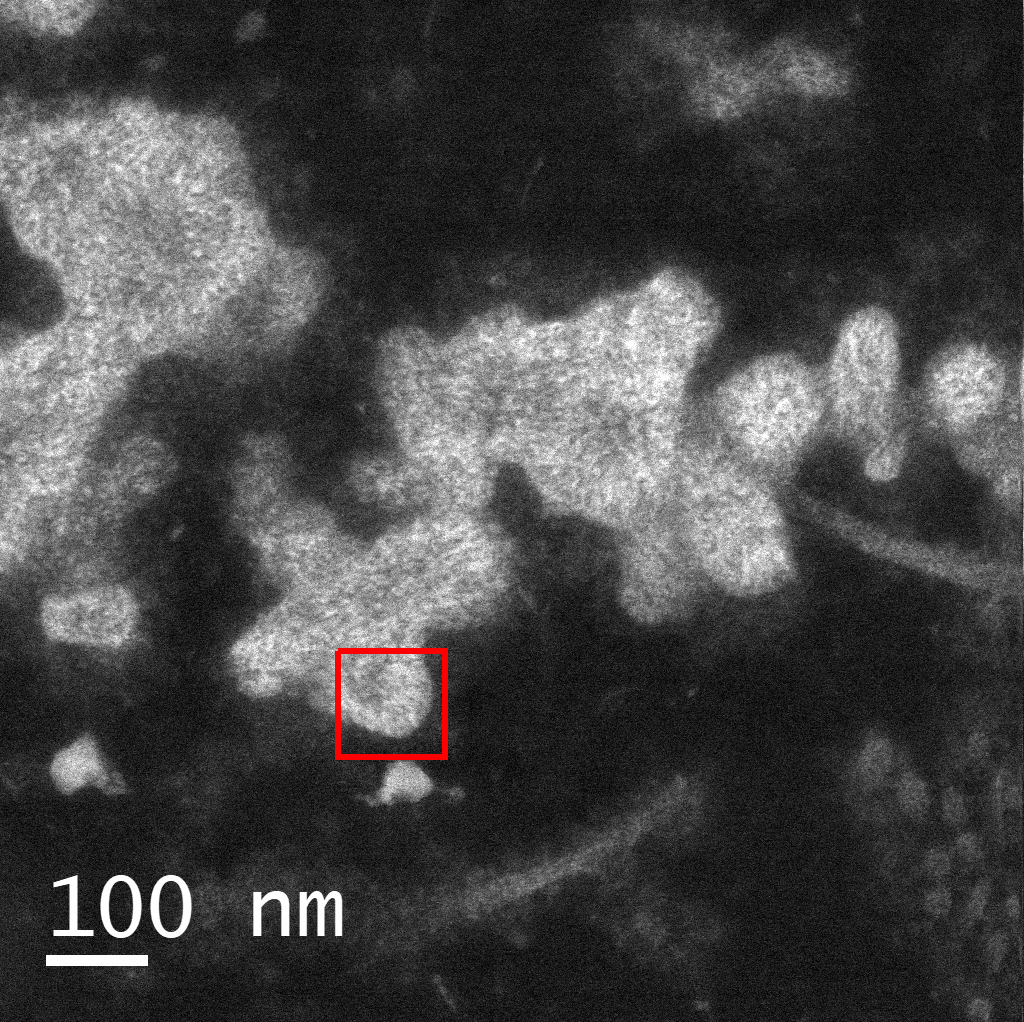
\includegraphics[height=0.5\textwidth]{img/chapitre3/figure1/haadf-LR-2.png}}
    \hspace{1em}
    \subfigure[\label{fig-BR-haadf-b}]%
    {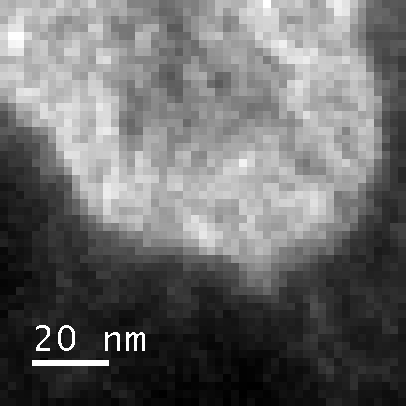
\includegraphics[height=0.35\textwidth]{img/chapitre3/figure1/haadf2.png}}\\
    %
    \caption{\protect\label{fig-BR-haadf}
        Images \gls{haadf} basse résolution d'un échantillon organique. 
        \subref{fig-BR-haadf-a} Acquisition \gls{haadf} avec prise de vue étendue afin de localiser la zone d'intérêt représentée en rouge. L'image est de taille 907$\times$907 pixels. 
        \subref{fig-BR-haadf-b} Acquisition \gls{haadf} prise en même temps que des données \gls{eels}. La résolution spatiale est donc la même. L'image est de taille 51$\times$51. 
    }
\end{figure}


\subsection{Images spatialement lisses en haute résolution}

Dans le chapitre~\ref{ch-chapter_4}, nous discuterons des images haute résolution à échelle atomique, tout particulièrement lorsque l'échantillon est cristallin et l'image est spatialement périodique.
%
Or, certains échantillons sont partiellement amorphes ou mal orientés si bien qu'aucune structure périodique ne peut être obtenue, comme c'est le cas sur la figure~\ref{fig-materiau-amorphe-a} pour des filaments d'ADN marqués à l'uranium et au thorium.
%
Ou encore, la forme du composé ne permet pas d'obtenir une image atomique définie, comme c'est le cas pour les nanotubes de carbone de la figure~\ref{fig-materiau-amorphe-b}.
%
Dans ces situations, l'image haute-résolution peut être suffisamment lisse pour être considérée dans le cadre applicatif de ce chapitre. Toutefois, les expériences menées n'utiliseront pas de telles images, mais des images basse résolution.  

\begin{figure}[h]
    \centering
    \subfigure[\protect\label{fig-materiau-amorphe-a}]{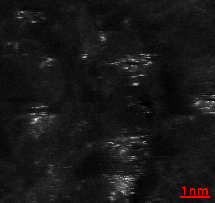
\includegraphics[height=5cm]{img/chapitre3/figure13/example-sc.png}}
    %
    \hspace{1em}
    %
    \subfigure[\protect\label{fig-materiau-amorphe-b}]{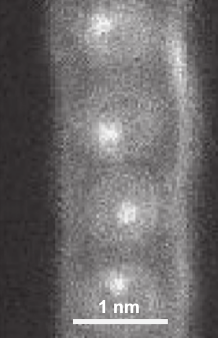
\includegraphics[height=5cm]{img/chapitre3/figure13/example3.png}}
    %
    \caption{Exemples d’images HAADF haute résolution ne présentant pas de structure atomique périodique. 
        \protect\subref{fig-materiau-amorphe-a} Atomes de Th et de Tb déposés sur un film de C amorphe très mince ($\approx$~\np[nm]{4} d'épaisseur)~\cite{march2014adressing}.
        \protect\subref{fig-materiau-amorphe-b} Métallo-fullerènes encapsulés dans des nanotubes de carbone~\cite{colliex2012capturing}.
        \protect\label{fig-materiau-amorphe}}
\end{figure}


\subsection{Information a priori et régularisations}\label{subsec-BR-reguls}

Dans le chapitre précédent, nous avons montré l'intérêt d'une technique par \gls{mc} régularisés en vue de reconstruire une image \gls{eels} sous-échantillonnée de manière efficace et rapide. Plus précisément, restituer un spectre-image complet \gls{X} à partir de mesures partielles \gls{Yi} est un problème inverse mal posé et la qualité de la méthode par \gls{mc} régularisés repose sur le choix de régularisations appropriées.
%
Les travaux présentés dans ce chapitre exploitent deux types différents d'information intrinsèque partagé par les données \gls{eels} spatialement lisses, à savoir la régularité spatiale et la propriété faible-rang dans le domaine spectral discutées ci-dessous.

\paragraph{Régularisations spatiales.} Dans le cadre applicatif de ce chapitre, les spectre-images \gls{eels} seront supposés spatialement lisses, que ce soit dû, par exemple, à une faible résolution de l'image ou à un échantillon amorphe. Par conséquent, on minimisera l'énergie du gradient de l'image \frobnorm{\nabla \gls{X}}, aussi appelé énergie de Sobolev, ce qui impose la régularité spatiale dans chaque bande.

\paragraph{Régularisations spectrales.} La \cref{sec-acp-redondance} a mis en lumière une propriété particulière des images multibandes telles que les images hyperspectrales issues de la télédétection ou encore les spectre-images \gls{eels} étudiés dans ce manuscrit, à savoir leur grande corrélation spectrale et la propriété faible-rang dans le domaine spectral. Cependant, promouvoir la structure faible-rang du spectre-image \gls{X} nécessite la minimisation du rang de \gls{X}, ce qui est un problème NP-difficile. Une alternative consiste à minimiser la norme nucléaire $||\gls{X}||_*$ définie comme la norme $\ell_1$ des valeurs singulières de \gls{X}. Cette relaxation convexe populaire conduit à un problème convexe facilement optimisable~\cite{recht2010guaranteed}.

Nous considérerons également une régularisation spectrale alternative basée sur une contrainte de sous-espace. En s'inspirant de stratégies déjà suivies dans \cite{wei2015bayesian} et \cite{wei2015fast} pour réaliser la fusion d'images multi-bandes, l'idée principale est d'estimer a priori le sous-espace linéaire où les spectres \gls{eels} évoluent et de reconstruire l'image complète dans ce sous-espace. Plus précisément, le sous-espace d'intérêt est d'abord estimé en appliquant une \gls{acp} aux données observées. Ensuite, le problème d'optimisation~\eqref{eq-MC-regul} est reformulé afin de projeter le spectre-image sur les composantes principales les plus puissantes. Les puissances des composantes principales sont de plus exploitées afin de définir une régularisation spectrale pondérée appropriée.

Les régularisations spatiale et spectrale décrites précédemment conduisent à deux formulations variationnelles différentes pour le problème de reconstruction de spectre-image \gls{eels}, qui sont détaillées dans les sections suivantes.

\newpage
%
\section{La méthode S2N}

\subsection{Formulation}\label{s2n-formulation}

\'Etant donné le modèle direct détaillé à la \cref{subsec-direct-inverse-problem} et les caractéristiques spatiale et spectrale du spectre-image \gls{eels} discutées à la \cref{subsec-BR-reguls}, la première méthode de reconstruction consiste à résoudre le problème d'optimisation suivant
\begin{equation}\label{eq-s2n}
    \gls{Xh} = \argmin_{\gls{X}\in\mathbb{R}^{\taille{M}{P}}} %
    %
    \frac{1}{2} \frobnorm{\gls{Yi} - \gls{X}_{\gls{I}}}  +
    \frac{\gls{ls2n}}{2} \frobnorm{\gls{X}\gls{D}} + 
    \gls{ms2n} ||\gls{X}||_*
\end{equation}
où \gls{D} est l'opérateur de gradient spatial discret appliqué à tous les canaux indépendamment. Ce problème d'optimisation appelé \gls{s2n} repose sur deux paramètres \gls{ls2n} et \gls{ms2n} ajustant respectivement les poids des régularisations spatiale et spectrale. Le choix de ces paramètres est discuté dans la section suivante.


\subsection{Estimation des paramètres de régularisation}\label{sec-s2n-param-tuning}

Nous allons à présent discuter le choix des paramètres \gls{ls2n} et \gls{ms2n} ajustant les régularisations spatiale et spectrale dans la fonction objectif de \gls{s2n} décrite à l'équation~\eqref{eq-s2n}. Afin d'ajuster correctement la paire de paramètres\footnote{Afin d'alléger les notations, les lettres \gls{s2n} en indice sont omises dans cette section.} $(\lambda,\mu)$, et en notant $y_{m,\gls{I}(n)}$ la $m$\textsuperscript{ème} composante du spectre  $\gls{Y}_{\gls{I}(n)}$ mesuré à la position spatiale indexée par $\gls{I}(n)$, la stratégie proposée repose sur l'hypothèse suivante
\begin{equation}
    \mathrm{E}\left[ \left(  y_{m,\gls{I}(n)} - x_{m,\gls{I}(n)}  \right)^2 \right] = \gls{sig}^2
\end{equation}
qui met en relation la variance du bruit $\gls{sig}^2$ avec l'erreur de reconstruction attendue en chaque bande et en chaque pixel.
%
Partant de cette hypothèse, choisir la solution optimale
$\gls{Xh}^{\textrm{opt}} \triangleq \gls{Xh}\left(\lambda^{\textrm{opt}}, \mu^{\textrm{opt}}\right)$
parmi l'ensemble de solutions possible 
$\left\{\gls{Xh}{\left(\lambda,\mu\right)}\right\}_{\lambda,\mu}$
consisterait à résoudre le problème suivant
\begin{equation}
\left(\lambda^{\textrm{opt}},\mu^{\textrm{opt}}\right) \in \operatornamewithlimits{argmin}_{(\lambda,\mu)\in\mathbb{R}_+^2} \mathcal{J}\left(\lambda,\mu\right)
\end{equation}
avec
\begin{equation}
\mathcal{J}\left(\lambda,\mu\right) \triangleq \left(\frac{1}{\gls{M}\gls{N}}\left\|\gls{Yi}-\gls{Xh}_{\gls{I}}{(\lambda,\mu)}\right\|_{\mathrm{F}}^2-\hat{\gls{sig}}^2\right)^2
\end{equation}
où $\hat{\gls{sig}}^2$ est une estimation de la variance du bruit (\cf\ \cref{subsec-formulation-3s}). Puisque la résolution du problème S2N est lourde d'un point de vue calculatoire, on préfère simplifier l'estimation de $\left(\lambda^{\textrm{opt}},\mu^{\textrm{opt}}\right)$ en fixant les paramètres de régularisation $(\lambda, \mu)$ comme suit
\begin{equation*}
\left\{
\begin{array}{cc}
\lambda^* &= c^\circ \lambda^{\circ} \\
\mu^*     &= c^\circ \mu^{\circ}
\end{array}
\right.
\end{equation*}
où $\lambda^{\circ}$, $\mu^{\circ}$ et $c^{\circ}$ sont successivement estimés en résolvant
\begin{align}
\lambda^{\circ} &\in \argmin_{\lambda\in\mathcal{G}_{\lambda}} \mathcal{J}(\lambda,0) \label{eq-adjust_lambdaS2N}\\
%
\mu^{\circ} &\in \argmin_{\mu\in\mathcal{G}_{\mu}} \mathcal{J}(0,\mu) \label{eq-adjust_muS2N}\\
%
c^\circ &\in \argmin_{c\in\mathcal{G}_c} \mathcal{J}(c\lambda^{\circ},c\mu^{\circ})\label{eq-adjust_cS2N}
\end{align} 
respectivement sur les grilles de recherches $\mathcal{G}_{\lambda}$, $\mathcal{G}_{\mu}$ et $\mathcal{G}_{c}$ construites dynamiquement à l'aide d'un processus dichotomique. 
Les deux premières étapes \eqref{eq-adjust_lambdaS2N} et \eqref{eq-adjust_muS2N} ajustent de manière indépendante les poids des régularisations spatiale et spectrale présentes dans la fonction coût \eqref{eq-s2n} de \gls{s2n}.
La troisième étape \eqref{eq-adjust_cS2N} vise à réajuster les paramètres $\lambda^{\circ}$ et $\mu^{\circ}$ afin de réduire l'impact des régularisations spatiale et spectrale considérés conjointement tout en préservant leurs proportions respectives dans l'équation~\eqref{eq-s2n}.

%
\section{La méthode 3S}

\subsection{Formulation}\label{subsec-formulation-3s}

Afin de promouvoir la propriété faible-rang du spectre-image \gls{eels} reconstruit, l'approche \gls{s2n} présentée dans la section précédente repose sur une pénalisation faible-rang induite par la norme nucléaire. A l'inverse, l'approche \gls{3s} décrite à présent impose cette propriété à l'aide d'une contrainte forte.
Plus précisément, l'image à recouvrer est supposée s'écrire $\gls{X} = \gls{H}\gls{S}$ où \gls{H} est une matrice orthonormale de taille \taille{M}{M} spécifiant la base des composantes principales propres aux données et $\gls{S}=[\mathbf{s}_1, \dots, \mathbf{s}_P]$ est une matrice de taille \taille{M}{P} rassemblant les coefficients de représentation associés aux spectres $\mathbf{x}_n$ dans cette base.
Dans ce contexte, la base \gls{H} est supposée être estimée a priori en appliquant une \gls{acp} aux données observées \gls{Yi}.
%
\`A noter que, comme expliqué à la \cref{sec-ech-sensibles}, le \gls{snr} obtenu en réalisant une acquisition partielle de la scène est supérieur à celui obtenu avec un échantillonnage conventionnel. Par conséquent, l'espace engendré par les premières composantes dont les puissances sont les plus élevées constitue une estimation fiable du véritable sous-espace signal (dont la dimension est notée \gls{Rt}).

\'Etant donné cette décomposition, la reconstruction du spectre-image \gls{X} peut être formulée directement dans la base des composantes principales et se réduit à l'estimation des \taille{M}{P} coefficients de la matrice \gls{S}. Par conséquent, le terme quadratique d'attache aux données $\frobnorm{\gls{Yi} - \gls{X}_{\gls{I}}}$ déjà utilisé dans le critère de \gls{s2n} peut être remplacé par $\frobnorm{\gls{Yi} - \gls{H}\gls{S}_{\gls{I}}}$ ou de manière équivalente, puisque \gls{H} est orthogonal, par $\frobnorm{\gls{H}^T\gls{Yi} - \gls{S}_{\gls{I}}}$. De la même manière, le terme $\frobnorm{\gls{X}\gls{D}}$ contraignant la régularité spatiale de l'image dans l'équation~\eqref{eq-s2n} peut être réécrit au moyen des coefficients de représentation $\frobnorm{\gls{S}\gls{D}}$.

De plus, lorsque les vecteurs propres $\mathbf{h}_1,\dots,\mathbf{h}_M$ identifiés par \gls{acp} et composant les colonnes de \gls{H} sont ordonnés par rapport aux valeurs propres triées par valeurs décroissantes, les vecteurs de représentation correspondants $\gls{S}_{1, :},\dots,\gls{S}_{M, :}$ sont supposés être de puissance décroissante, où $\gls{S}_{m, :}$ désigne la $m$\textsuperscript{ième} ligne de \gls{S}. En particulier, si les spectres de l'image évoluent dans un sous-espace de dimension \gls{Rt} avec $\gls{Rt}\leq\gls{M}$, la norme quadratique des vecteurs de représentation non pertinents est supposé être proche de 0 pour $m>\gls{Rt}$. Cela suggère une pénalisation pondérée de la forme $\sum_{m=1}^{M}w_m||\gls{S}_{m, :}||_2^2$ avec des poids croissants $(w_m)_{m=1,\dots,M}$.
%
Le dimensionnement des poids qui sera discuté à la section suivante suggère que $w_m$ soit infini pour $m>\gls{R}$ où \gls{R} est une estimation de la véritable dimension \gls{Rt} ($\gls{R}\leq\gls{M}$). Cette règle implique systématiquement que $\gls{S}_{m, :}$ soit un vecteur nul pour $m> \gls{R}$. En d'autres termes, le problème d'optimisation \gls{3s} peut être écrit de manière équivalente par rapport à une matrice $\gls{S}_{1:R, :}$ de taille \taille{R}{P}.

Finalement, l'approche \gls{3s} proposée consiste à résoudre le problème d'optimisation suivant
\begin{align}
\hat{\gls{S}} &= \argmin_{\gls{S}\in\mathbb{R}^{\taille{R}{P}}}
    %
    \frac{1}{2\gls{R}}\frobnorm{\gls{S} \gls{D}} + 
    \frac{\gls{m3s}}{2}\sum_{m=1}^{\gls{R}} w_{m} \twonorm{\gls{S}_{m,:}} \nonumber \\
%
&\textrm{s.t.}\quad         
    \frac{1}{\gls{R}}\twonorm{\gls{H}_{1:\gls{R}}^T\mathbf{y}_{\gls{I}(n)}-\mathbf{s}_{\gls{I}(n)}}
    \leq\gls{hsig}^2,\ \forall n\in\llbracket 1, \gls{N} \rrbracket \label{eq-3s}
\end{align}
où \gls{m3s} est un paramètre permettant d'ajuster l'impact des régularisations spatiale et spectrale et où $\gls{H}_{1:\gls{R}}$ correspond à la matrice de taille \taille{M}{R} contenant les \gls{R} premières colonnes de \gls{H}. Dans l'équation~\eqref{eq-3s}, le terme d'attache aux données dans \eqref{eq-MC-regul} est converti en une contrainte puisque la distance euclidienne au carré entre les observations et la solution est supposée être bornée par la variance du bruit $\gls{sig}^2$.
%
La borne peut être supérieure à $\gls{sig}^2$, elle peut valoir par exemple $\frac{1}{R}F_{\chi^2}^{-1}(1-\alpha)\sigma^2$ où $F_{\chi^2}$ est la fonction cumulative de la loi du $\chi^2$ et $\alpha$ est la probabilité de ne pas respecter la contrainte quand bien même les éléments de $\gls{H}_{1:\gls{R}}^T\mathbf{y}_{\gls{I}(n)}-\mathbf{s}_{\gls{I}(n)}$ suivent réellement une loi gaussienne centrée de variance $\sigma^2$. En pratique, lorsque l'on augmente la borne, l'image reconstruite produite est davantage lissée et  choisir $\sigma^2$ comme borne produit des résultats visuellement meilleurs.
%

En pratique, une estimation $\gls{hsig}^2$ de la variance du bruit  $\gls{sig}^2$ et une estimation \gls{R} de \gls{Rt} peuvent être obtenus à partir d'une décomposition en éléments propres de la matrice de covariance empirique des observations (\cf\ sections~\ref{subsec-3s-poids} et \ref{subsec-3s-acp}). L'image reconstruite est finalement définie comme\footnote{Afin d'alléger l'écriture, et ce malgré un léger abus de notations, les indices $\cdot_{1:\gls{R}}$ et $\cdot_{1:\gls{R}, :}$ seront omis dans la suite du chapitre.} $\gls{Xh} = \gls{H}_{1:\gls{R}}\gls{S}_{1:\gls{R}, :}$.
Il y a un triple avantage à formuler le problème de reconstruction comme énoncé ci-dessus. 
%
D'abord, l'ACP impose explicitement une structure faible rang du spectre-image à reconstruire (comme le fait la norme nucléaire pour S2N). Ensuite, comme cela sera vu dans la \cref{subsec-implementation-3s} concernant l'implémentation de \gls{3s}, elle réduit fortement la charge calculatoire de l'algorithme de minimisation résultant puisque $R$ est censé être significativement inférieur à $M$ et, contrairement à S2N, il n’y a plus besoin de réaliser une SVD. Enfin, la norme nucléaire n'est pas une relaxation optimale du rang puisqu'elle biaise fortement les données.


\subsection{Estimation des poids et de la dimension du sous-espace}\label{subsec-3s-poids}

Comme expliqué auparavant, les vecteurs $\mathbf{h}_1,\ldots,\mathbf{h}_{\gls{R}}$ générant le sous-espace d'intérêt sont supposés être ordonnés par rapport aux valeurs propres correspondantes $\gls{d}_1\geq\gls{d}_2\geq \ldots\geq \gls{d}_{\gls{M}}$ triées par ordre décroissant. En particulier, puisque les données sont faible rang, les dernières directions correspondent au bruit. Par conséquent, les vecteurs de représentation $(\gls{S}_{m, :})_{m=1,\dots,\gls{M}}$ sont supposés être moins pertinents à mesure que $m$ augmente. Le choix des poids $(\gls{w}_{m, :})_{m=1,\dots,\gls{M}}$ s'inspire de cette observation, en l'interprétant dans un cadre bayésien.
%
Plus précisément, supposons que la matrice d'observation \gls{Yi} peut être liée dans le cas d'un échantillonnage complet au spectre-image inconnu \gls{X} par le modèle standard de débruitage
\begin{equation}
    \gls{Y} = \gls{X} + \gls{E}
\end{equation}
où \gls{E} est une matrice de bruit de taille \taille{M}{N}. Ce modèle d'acquisition peut être reformulé dans le sous-espace signal comme
\begin{equation}\label{eq-weights-sp-model}
    \gls{H}^T\gls{Y} = \gls{S} + \mathbf{N}
\end{equation}
avec $\mathbf{N} \triangleq \gls{H}^T\gls{E}$. Dans~\eqref{eq-weights-sp-model}, $\mathbf{N}$ représente une matrice de perturbations dont les lignes $(\mathbf{N}_{m, :})_{m=1,\dots,\gls{M}}$ sont supposées être indépendantes et identiquement distribuées (i.i.d.) selon la distribution normale
\begin{equation}
    \mathbf{N}_{m, :} \sim \mathcal{N}\left(\boldsymbol{0}_{\gls{N}},\gls{sig}^2 \mathds{1}_{\gls{N}}\right).
\end{equation}
Les lignes $(\gls{S}_{m, :})_{m=1,\dots,\gls{M}}$ de \gls{S} sont supposées i.i.d. et on leur assigne la distribution gaussienne conjuguée suivante
\begin{equation}
    \gls{S}_{m,:} \sim \mathcal{N}\left(\boldsymbol{0}_{\gls{N}},\eta^2_{m} \mathds{1}_{\gls{N}}\right).
\end{equation}
Calculer l'estimateur du \gls{map} de \gls{S} consiste à résoudre
\begin{equation}
\argmin_{\gls{S}} \frobnorm{\gls{H}^T\gls{Y}-\gls{S}} + \sum_{m = 1}^{\gls{M}} \frac{\gls{sig}^2}{\eta^2_m}\twonorm{\gls{S}_{m,:}}.
\label{eq-3S_OP_2_Bayesian}
\end{equation}
En comparant le problème \gls{3s}~\eqref{eq-3s} avec la formulation du MAP~\eqref{eq-3S_OP_2_Bayesian}, un choix naturel pour les poids $\gls{w}_m$ est
\begin{equation}
    \gls{w}_m = \frac{\gls{sig}^2}{\eta_m^2}. 
\end{equation}
Cependant, les variances $\eta_m$ des composantes $(\gls{S}_{m, :})_{m=1,\dots,\gls{M}}$ sont inconnues en pratique. Afin d'ajuster ces hyperparamètres, une solution consiste à recourir à une approche bayésienne empirique en étudiant la covariance du modèle linéaire~\eqref{eq-weights-sp-model}, ce qui conduit simplement à
\begin{equation}
    \gls{d}_m = \eta_m^2 + \gls{sig}^2
\end{equation}
où $\gls{d}_m$ peut être approché pour tout $m$ par la valeur propre empirique estimée par \gls{acp}. Toutefois, il est important de rappeler que, dans le cadre applicatif de cette étude, le nombre de canaux \gls{M} est généralement du même ordre de grandeur que le nombre d'échantillons \gls{N}. Ainsi, l'\gls{acp} conduite afin d'estimer les valeurs propres $\gls{d}_1, \dots, \gls{d}_M$ pourrait souffrir d'un manque d'échantillons et celle-ci fournirait des estimées  peu fiables. Afin d'améliorer cette estimation, la section suivante propose une correction à appliquer aux valeurs propres issues de l'\gls{acp}. Finalement, $\gls{d}_m$ est approché par $\hat{d}_m^2$ et estimée par \gls{acp} après que la correction détaillée dans la \cref{subsec-3s-acp} ait été appliquée. D'autre part, l'estimée $\gls{hsig}^2$ de $\gls{sig}^2$ est définie comme la valeur propre corrigée $\hat{d}_m^2$ minimale (dont la multiplicité peut être supérieure à un). Les poids sont finalement choisis comme
\begin{equation}\label{eq-weights-form}
    \gls{w}_m = \frac{\gls{hsig}^2}{\hat{d}_m^2 - \gls{hsig}^2}.
\end{equation}
Une illustration de la dépendance entre $\hat{d}_m^2$ et $\gls{w}_m$ est donnée à la \cref{fig-S_constraint}. 

De plus, la règle~\eqref{eq-weights-form} suggère aussi la définition d'une estimée \gls{R} de la dimension du sous-espace signal réel \gls{Rt} comme l'indice $m$ maximum tel que $\hat{d}_{m}^2 > \gls{hsig}^2$. Pour $m=\gls{R}+1, \dots, \gls{M}$, les poids sont fixés  à $\gls{w}_m = \infty$ puisque les vecteurs de représentation correspondants ne sont censés être composés de bruit uniquement. Par conséquent, ces composantes $(\mathbf{s}_m)_{m=\gls{R}+1,\dots,\gls{M}}$ sont contraintes à être nulles et le problème d'optimisation~\eqref{eq-3s} de \gls{3s} peut être reformulé afin de minimiser par rapport à une matrice de taille \taille{R}{P}.

\begin{figure}[ht]
    \centering
    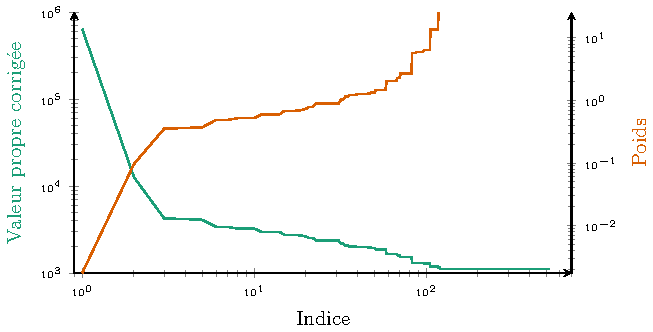
\includegraphics[width=0.8\columnwidth]{img/chapitre3/figure2/weights_curve.pdf}
    \caption{Une représentation des valeurs propres corrigées (tracé vert) et des poids associés (tracé orange). Un spectre-image réel a été utilisé ici. Les poids d'indice supérieur à 112 sont infinis puisque $\hat{\sigma}$ et $(\hat{d}^2_{m})_{m=112,\dots,\gls{M}}$ sont égaux.
        \protect\label{fig-S_constraint}}
\end{figure}


\subsection{Correction des valeurs propres estimées par ACP}\label{subsec-3s-acp}

La technique d'estimation des poids de \gls{3s} détaillée à la section précédente requiert une estimation des variances $\gls{d}_1,\dots,\gls{d}_{\gls{M}}$ des composantes du signal dans la base des colonnes de \gls{H}. Quand \gls{H} est identifié par \gls{acp}, cette estimation est généralement réalisée en appliquant une décomposition en éléments propres de la matrice de covariance empirique des spectres observés, \ie{},
\begin{equation}
    \hat{\boldsymbol\Sigma} = \frac{1}{\gls{N}}\gls{Yi}\gls{Yi}^T = \mathbf{H}\mathbf{G}\mathbf{H}^T
\end{equation}
où $\mathbf{G} = \mathrm{diag}(\tilde{d}_1^2, \dots, \tilde{d}_{\gls{M}}^2)$. \`A noter que les valeurs propres empiriques sont triées par ordre décroissant et sont positives, \ie{}, $\tilde{d}_1^2 \geq \tilde{d}_2^2 \geq \dots \geq \tilde{d}_{\gls{M}}^2\geq 0$. Le défaut principal de cet estimateur simple est qu'il est construit afin de donner une estimée fiable quand le nombre d'échantillons \gls{N} est suffisamment grand par rapport à la dimension des observations \gls{M}. Toutefois, ce n'est pas le cas de notre contexte applicatif puisque \gls{N} est du même ordre de grandeur que \gls{M}. Plusieurs stratégies ont été proposées dans la littérature afin d'améliorer l'estimation des valeurs propres. Afin de corriger les valeurs propres empiriques, une alternative consiste à avoir recours à l'estimateur de Stein défini comme~\cite{mestre2008improved}
\begin{equation}\label{eq-Stein-corr}
\hat{d}^2_m = 
\frac{\tilde{d}^2_m}{1+ \frac{1}{N}\sum_{\substack{j=1\\j\neq m }}^M \frac{\tilde{d}^2_m+\tilde{d}^2_j}{\tilde{d}^2_m-\tilde{d}^2_j}}.
\end{equation}
Cependant, cet estimateur n'impose pas la propriété de non-croissance et quelques valeurs propres corrigées $(\hat{d}_m)_{m=1,\dots,\gls{M}}$ peuvent être négatives. Pour corriger ce problème, une régression isotonique a été proposée dans~\cite{LinPerl1985} comme post-traitement. Cette procédure détaillée à l'annexe~\ref{abstr-regression-isotonique} renvoie généralement un ensemble de valeur propres corrigées et leur multiplicités associées. De plus, une estimation $\gls{hsig}^2$ de la variance du bruit $\gls{sig}^2$ requise dans la définition des poids~\eqref{eq-weights-form} peut être définie comme la valeur propre corrigée de valeur minimale dont la multiplicité est $\gls{M} - \gls{R}$.

%
\section{Implémentation}\label{ch-3-implementation}

Cette section décrit les algorithmes pour résoudre les problèmes d'optimisation~\eqref{eq-s2n} et \eqref{eq-3s}. Tous deux reposent sur l'algorithme \gls{fista}~\cite{beck_fast_2009} dont la formulation générique est rappelée dans la section suivante.

\subsection{L'algorithme FISTA}\label{sec-fista}

Afin d'implémenter les méthodes proposées, le problème d'optimisation générique à résoudre est de la forme
\begin{equation}
\hat{x} = \argmin_x f(x) + g(x) \label{eq:GeneralOP}
\end{equation}
\begin{itemize}
    \item $f : \mathbb{R}^p \to \mathbb{R}$ est une fonction convexe, continuellement différentiable dont le gradient est continu et $L_{f}$-Lipschitz,
    \item $g : \mathbb{R}^p \to \mathbb{R}$ une fonction convexe possiblement non-lisse.
\end{itemize}
Une méthode basique d'ordre un (\ie{}, ne nécessitant d'évaluer que les fonctions et leur gradient) est l'algorithme \gls{ista} basé sur une itérée de la forme
\begin{equation}
    x^{(i+1)} \leftarrow \mathrm{prox}_{g}( \nabla f(x^{(i)})).
\end{equation}
où $\mathrm{prox}_{g}$ est l'opérateur proximal associé à $g(\cdot)$. Seulement, le taux de convergence de cette méthode est faible, à savoir
\begin{equation}
(f+g)(x^{(i+1)}) - (f+g)(x^{(i)}) \approx \mathcal{O}(1/i).
\end{equation}
Pour accélérer cette méthode, les travaux de Nesterov~\cite{nesterov1983method} ont conduit à un algorithme \guillemets{optimal} d'ordre un convergeant en $\mathcal{O}(1/i^2)$ à condition que $f$ et $g$ soient \emph{lisses}. Enfin, l'algorithme \gls{fista} proposé par Beck et Teboulle affiche un taux de convergence identique pour une fonction $g$ possiblement non-lisse et sera utilisé pour implémenter les méthodes S2N et 3S. En particulier, pour tout $L> L_{f}$, l'algorithme \gls{fista} donné à l'algorithme~\ref{algo-FISTA} converge vers une solution de ~\eqref{eq:GeneralOP}.

Les implémentations spécifiques aux problèmes~\eqref{eq-s2n} et \eqref{eq-3s} considérés sont présentées dans les sections suivantes.

\begin{algorithme}
    \begin{minipage}{\textwidth}
        \begin{algorithm}[H]
            \SetKwInOut{Input}{Entrée}
            \SetKwInOut{Init}{Initialisation}
            \Input{$L> L_{f}$ une borne supérieure de $L_{f}$}
            \Init{Fixer $\mathbf{y}^{(1)} = \mathbf{x}^{(0)} \in \mathbb{R}^p$, $\theta^{(1)}=1$, $i=1$}
            \While{critère d'arrêt n'est pas satisfait}{
                $\mathbf{x}^{(i)} = \mathrm{prox}_{g/L}\left( \mathbf{y}^{(i)}-\frac{1}{L}\nabla f(\mathbf{y}^{(i)}) \right)$\label{LigneAlgo1} \nllabel{algostep:gradient}\;
                $\theta^{(i+1)} = \frac{1}{2} \left(1+\sqrt{1+4(\theta^{(i)})^2}\right)$\nllabel{LigneAlgo2}\;
                $\mathbf{y}^{(i+1)} = \mathbf{x}^{(i)} + \left( \frac{\theta^{(i)}-1}{\theta^{(i+1)}} \right) \left(\mathbf{x}^{(i)}-\mathbf{x}^{(i-1)} \right)$\nllabel{LigneAlgo3}\;
                $i \leftarrow i+1$\nllabel{LigneAlgo4}
            }
        \end{algorithm}
    \end{minipage}
    \caption[][-1em]{FISTA avec un pas constant \cite{beck_fast_2009}.\protect\label{algo-FISTA}}
\end{algorithme}

\subsection{Application à S2N}

Afin de résoudre~\eqref{eq-s2n}, la méthode \gls{s2n} consiste à adopter la décomposition suivante
\begin{align}
    f(\gls{X}) &= \frac{1}{2}\frobnorm{\gls{Yi}-\gls{X}_{\gls{I}}} + \frac{\gls{ls2n}}{2}\frobnorm{\gls{X} \gls{D}}\\
    g(\gls{X}) &= \gls{ms2n} \left\|\gls{X}\right\|_*.
\end{align}
Le gradient associé à $f(\cdot)$ requis à la ligne \ref{algostep:gradient} de l'algorithme~\ref{algo-FISTA} est donné par
\begin{equation}
    \label{nablaf-s2n}
    \nabla f(\gls{X}) = (\gls{X}\gls{Phi} - \gls{Yi})\gls{Phi}^T - \gls{ls2n} \gls{X} \Delta
\end{equation}
où $\Delta = -\gls{D}\gls{D}^T$ est l'opérateur de laplacien spatial discret et \gls{Phi} est l'opérateur de sous-échantillonnage tel que $\gls{X}_{\gls{I}} = \gls{X}\gls{Phi}$.
Une borne supérieure de $L_f$ est obtenu par
\begin{equation}
    ||\nabla f(\gls{X})||\leq (\underbrace{1+\gls{ls2n} \left\|\Delta\right\|}_{L})\ ||\gls{X}||
\end{equation}
où $\left\|\Delta\right\|$ est la norme spectrale de l'opérateur de laplacien spatial discret, qui vaut 8 en dimension 2. Une borne supérieure de la constante de Lipschitz associée à $\nabla f$ est donc $L= 1 +8\gls{ls2n}$. 

De plus, en notant $\gls{X}=\mathbf{U}\boldsymbol{\Sigma} \mathbf{V}^T$ la décomposition en valeurs singulières de \gls{X}, où $\boldsymbol{\Sigma} = \mathrm{diag}(\mu_i)$, l'opérateur proximal associé à $g(\cdot)$ est~\cite{cai1956singular}
\begin{align}
    \mathrm{prox}_{g/L}(\gls{X}) &\triangleq \argmin_{\mathbf{T}} 
                                    \left\{ \frac{g(\mathbf{T})}{L} + \frac{1}{2}\frobnorm{\mathbf{T} - \gls{X}} \right\}\\
                               &= {\mathbf{U}} \bar{\boldsymbol{\Sigma}} {\mathbf{V}}^T, \label{prox-s2n}
\end{align}
où $\bar{\boldsymbol{\Sigma}} = \mathrm{diag}(\bar{\mu}_i)$ contient les valeurs singulières après seuillage doux de seuil \gls{ms2n}, \ie{}
\begin{equation}
    \bar{\mu}_i = \mathrm{sgn}(\mu_i)\left(|\mu_i|-\frac{\gls{ms2n}}{L}\right)\iota_{\mu_i>\gls{ms2n}}(\mu_i)
\end{equation}
où $\mathrm{sgn}$ est la fonction signe et où $\iota$ est la fonction indicatrice.

Le pseudo-code complet permettant l'implémentation de S2N avec ou sans recherche de paramètres optimaux est disponible à l'annexe~\ref{annexe-implementation-3s-s2n}.


\subsection{Application à 3S}\label{subsec-implementation-3s}

Concernant le problème~\eqref{eq-3s}, la méthode \gls{3s} proposée repose sur la décomposition suivante
\begin{align}
    f(\gls{S}) &= 
    \frac{1}{2\gls{R}}\frobnorm{\gls{S} \gls{D}} + 
    \frac{\gls{m3s}}{2}\sum_{m=1}^{\gls{R}} \gls{w}_{m} \twonorm{\gls{S}_{m,:}}\\
    %
    g(\gls{S}) &= 
    \sum_{n=1}^{\gls{N}} \iota_{
        \mathcal{B}(\gls{H}^T\mathbf{y}_{\gls{I}(n)},\sqrt{\gls{R}}\gls{hsig})
    }(\mathbf{s}_{\gls{I}(n)})
    \label{eq-3S_g}
\end{align}
où
\begin{equation}
    \iota_\mathcal{A}(x) = \left\{\begin{array}{lr}
    0,        & \text{if } x\in   \mathcal{A}\\
    +\infty, & \text{if } x\notin\mathcal{A}
    \end{array}\right.
\end{equation}
est la fonction indicatrice relative à l'ensemble $\mathcal{A}$ et $\mathcal{B}(x_0,r)$ est la boule fermée en norme $\ell_2$ de centre $x_0$ et de rayon $r$.
Le gradient de $f(\cdot)$ est
\begin{equation}\label{nabla-f-3s}
    \nabla f(\gls{S}) = -\frac{1}{\gls{R}} \gls{S}\Delta + \gls{m3s}\mathbf{W}\gls{S}\\
\end{equation}
où $\mathbf{W}=\mathrm{diag}\left\{w_1,\ldots,w_{\gls{R}}\right\}$ est la matrice diagonale contenant les poids.
De manière similaire à \gls{s2n}, une borne supérieure de $L_f$ est obtenue par
\begin{equation}
||\nabla f(\gls{S})|| \leq 
(\underbrace{\left\|\Delta\right\| + \gls{m3s}\left\|\mathbf{W}\right\|}_{L})
\ ||\gls{S}||
\end{equation}
conduisant à $L = 8+\gls{m3s}\max_{m}\left\{\gls{w}_{m}\right\}$.

De plus, comme nous le voyons à l'équation~\eqref{eq-3S_g}, la fonction $g(\cdot)$ est séparable relativement aux indices des pixels $n \in \llbracket 1,\gls{N}\rrbracket$. Par conséquent, l'opérateur proximal associé à $g(\cdot)$ consiste à projeter $\mathbf{s}_{\gls{I}(n)}$ sur $\mathcal{B}(\gls{H}^T\mathbf{y}_{\gls{I}(n)},\sqrt{\gls{R}}\gls{hsig})$ pour tout $n\in \llbracket 1,\gls{N}\rrbracket$.

Le pseudo-code complet permettant l'implémentation de 3S avec ou sans recherche de paramètres optimaux est disponible à l'annexe~\ref{annexe-implementation-3s-s2n}.

\subsection{Etude de la complexité}

Cette partie discute de la complexité algorithmique des méthodes \gls{s2n} et \gls{3s} en analysant le schéma algorithmique de \gls{fista} (algorithme~\ref{algo-FISTA}).

D'abord, les lignes~\ref{LigneAlgo2} et~\ref{LigneAlgo4} sont clairement de complexité asymptotique $\mathcal{O}(1)$. Ensuite, concernant la ligne~\ref{LigneAlgo3}, qui ne consiste qu'en une addition de matrices, la complexité est de l'ordre e $\mathcal{O}(\gls{M}\gls{P})$ pour \gls{s2n} et $\mathcal{O}(\gls{R}\gls{P})$ pour \gls{3s}. La ligne~\ref{LigneAlgo1} consiste en une étape de descente de gradient, suivie par un opérateur proximal. Le détail est donné à la \tabname~\ref{table-ComplexitySummary}. Cette étude montre que \gls{s2n} est plus lourd que \gls{3s} d'un point de vue calculatoire, principalement car \gls{s2n} requiert une décomposition en valeurs singulières à chaque itération, tandis que \gls{3s} opère sur une matrice de dimension réduite puisque $\gls{R} \leq \gls{M}$.

En plus de la complexité algorithmique étudiée ci-dessus, les temps d'exécution requis pour reconstruire le spectre-image réel utilisé à la \cref{sec-3s-real-data} sont donnés à la \tabname~\ref{table-ComplexitySummary} pour une implémentation non-optimisée sur un ordinateur équipé d'un CPU Intel Xeon de fréquence \np[GHz]{3,70} et de \np[Go]{15.6} de RAM. Ces résultats montrent que \gls{3s} est environ 1300 fois plus rapide que \gls{s2n} pour reconstruire ce spectre-image pour lequel $\gls{M}\gls{P}^2 \approx 10^9$ et $\gls{R}\gls{P} \approx 3\times 10^5$.

\begin{table}[h!]
    \centering
    \bgroup
    \def\arraystretch{1.5}
    \begin{tabular}{b{5cm}cc}
        \toprule
        Line&S2N&3S\\
        \midrule
        Line~\ref{LigneAlgo1} (gradient descent)        &$\mathcal{O}(\gls{M}\gls{P})$      &$\mathcal{O}(\gls{R} \gls{P})$\\
        Line~\ref{LigneAlgo1} (proximal operator)       &$\mathcal{O}(\gls{M}\gls{P}^2)$    &$\mathcal{O}(\gls{R} \gls{N})$\\
        Line~\ref{LigneAlgo3}                           &$\mathcal{O}(\gls{M}\gls{P})$      &$\mathcal{O}(\gls{R}\gls{P})$\\
        Lines~\ref{LigneAlgo2} and~\ref{LigneAlgo4}     &$\mathcal{O}(1)$           &$\mathcal{O}(1)$\\
        % \midrule
        TOTAL&$\mathcal{O}(\gls{M}\gls{P}^2)$    &$\boldsymbol{\mathcal{O}(\gls{R} \gls{P})}$\\
        \bottomrule
        Temps d'exécution de l'algo. (s)&237&\textbf{0.18}\\
        \bottomrule
    \end{tabular}
    \egroup
    \caption{Complexité d'une itération des algorithmes S2N et 3S. Les meilleurs scores sont en gras.
        \protect\label{table-ComplexitySummary}}
\end{table} 

%
\section{Résultats sur des données synthétiques}

\subsection{Création de données synthétiques}\label{sec-synth-data-lr}

Les performances des méthodes proposées sont évaluées à l'aide d'expériences conduites sur des données synthétiques. Plus précisément, les méthodes proposées sont appliquées au spectre-image complet $\gls{Y}\in\mathbb{R}^{\taille{M}{P}}$ généré selon le modèle
\begin{equation}
    \gls{Y} = \gls{X} + \gls{E}
\end{equation}
où \gls{X} est le spectre-image non bruité et \gls{E} est la matrice de bruit gaussien.
Afin de mimer une aquisition synthétique réaliste, l'image idéale \gls{X} est obtenue par mélange linéaire suivant le modèle $\gls{X} = \mathbf{M}\mathbf{A}$ donné à la section~\ref{sec-demelange} qui décrit la répartition spatiale de matériaux au sein d'un échantillon observé. La matrice $\mathbf{M}=[\mathbf{m}_1, \dots, \mathbf{m}_{N_c}]$ de taille $M\times N_c$ rassemble les $N_c$ spectres associés aux endmembers et $\mathbf{A} = [\mathbf{a}_1, \dots, \mathbf{a}_P]$ de taille $N_c\times P$ correspond aux abondances des endmembers pour chaque pixel.

\paragraph{Choix de la matrice d'endmembers $\mathbf{M}$.} Simuler un spectre EELS complet avec différents seuils et des structures fines associées à chaque seuil est compliqué. C'est pourquoi des spectres représentatifs $\mathbf{m}_1,\dots,\mathbf{m}_{N_c}$ ont été directement extraits de données réelles déjà étudiées pour leur intérêt médical : une section de rein (tissu biologique) incrustée dans une résine et contenant des calcifications~\cite{gay2020nanoscale}. Pour des échantillons biologiques aussi complets, le nombre d'endmembers $N_c$ doit être ajusté pour chaque jeu de données et est généralement compris entre 3 et 5. Ici, le nombre d'endmembers extraits est fixé à $N_c=4$. L'extraction des endmembers est réalisée en utilisant l'algorithme VCA~\cite{nascimento2005vertex}, un algorithme d'extraction d'endmember populaire initialement développé pour l'imagerie hyperspectrale mais qui est maintenant fréquemment utilisé dans la communauté \gls{eels}, sa description est donnée à la section~\ref{sec-demelange}.
%
Les spectres sont représentés à la figure~\ref{fig-spectres-synth} où quatre seuils caractéristiques révèlent la présence d'éléments particuliers : carbone ($K$-seuil à 285~eV), calcium ($L_{2,3}$-seuil à 350~eV), azote ($K$-seuil à 400~eV) et oxygène ($K$-seuil à 530~eV). Ces composantes ne correspondent pas à des composés chimiques bien déterminés. Néanmoins, pour plus de simplicité, par la suite, les endmembers vont être associés à des matériaux particuliers et seront désignés sous les noms de calcification (avec le seuil Ca-$L_{2, 3}$), résine, organique 1 (avec le seuil N-$K$) et organique 2. Le nombre de bandes (correspondant au nombre de canaux du spectromètre) est $M=\np{1337}$.


\begin{figure}[h!]
    \centering
    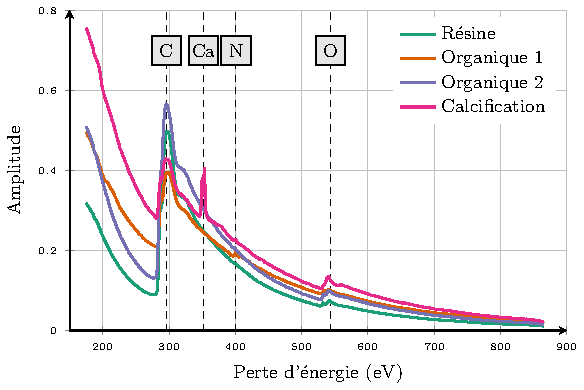
\includegraphics{img/chapitre3/figure4/endmember_spectra.pdf}
    \caption{Les $N_c=4$ spectres des endmembers représentant l'amplitude en fonction de la perte d'énergie (en eV). Les seuils caractéristiques suivants sont représentés : carbone (285~eV), calcium (350~eV), azote (400~eV) et oxygène (530~eV).
        \protect\label{fig-spectres-synth}}
\end{figure}


\paragraph{Choix de la matrice d'abondance $\mathbf{A}$.} Le coefficient $a_{k,p}$ donne la proportion du $k$\textsuperscript{ième} endmember au $p$\textsuperscript{ième} pixel. Afin de s'assurer d'une description additive cohérente du spectre-image à l'aide des $N_c$ matériaux introduite ci-dessus, ces coefficients sont contraints à être non-négatifs et à respecter l'hypothèse de somme à un telle que décrite aux équations~\eqref{eq-positivity} et~\eqref{eq-sum-to-one}, à savoir 
\begin{align}
&a_{k,p} \geq 0,\quad\forall p \in \llbracket 1,P \rrbracket,\forall k\in\llbracket 1,n_c\rrbracket\\
&\sum_k a_{k,p} = 1 \quad \forall p\in\llbracket 1 , N \rrbracket .
\end{align}
En respectant ces contraintes, quatre cartes d'abondance $(\mathbf{A}_{k, :})_{k=1,\dots,N_c}$ représentées à la figure~\ref{fig-cartes-abondance-synth} ont été construites pour définir la distribution spatiale des différents matériaux au sein de l'échantillon. Dans ces expériences, les cartes spatiales sont de taille $100\times 100$, ce qui correspond à $P=10^4$.

\begin{figure}[h!]
    \centering
    \subfigure[Résine]{
        
\includegraphics[width=0.2\textwidth]{img/chapitre3/figure4/Map1.png} }\hspace{0.1\textwidth}
    \subfigure[Organique 1]{
        
\includegraphics[width=0.2\textwidth]{img/chapitre3/figure4/Map2.png} }\\
    \subfigure[Organique 2]{
        
\includegraphics[width=0.2\textwidth]{img/chapitre3/figure4/Map3.png} }\hspace{0.1\textwidth}
    \subfigure[Calcification]{
        
\includegraphics[width=0.2\textwidth]{img/chapitre3/figure4/Map4.png} }
    %
    \caption{Les cartes d'abondance utilisées pour générer les données synthétiques. Les coefficients dont l'abondance vaut zero (resp. un) apparaissent en noir (resp. blanc), ce qui correspond à l'absence de l'endmember correspondant (resp. des autres endmembers).
        \protect\label{fig-cartes-abondance-synth}}
\end{figure}

\paragraph{Tirage de la matrice de bruit $\mathbf{E}$.} Les éléments de la matrice de bruit $\mathbf{E}$ sont tirés indépendamment et identiquement suivant une loi gaussienne centrée. La variance du bruit a été ajustée afin d'atteindre des valeurs de \gls{snr} réalistes détaillées plus loin.

\subsection{Métriques et mesures de vraisemblance}\label{sec-metriques}

Afin d'évaluer la qualité de reconstruction, plusieurs mesures quantitatives seront utilisées afin de comparer la vérité terrain \gls{X} avec l'image reconstruite \gls{Xh}. D'abord, l'erreur quadratique moyenne normalisée (\gls{nmse}) est choisie comme erreur de mesure et est définie par
\begin{equation}
    \mathrm{NMSE}(\gls{Xh}, \gls{X}) = \frac{\frobnorm{\gls{Xh} - \gls{X}}}{\frobnorm{\gls{X}}}.
\end{equation}
Ainsi, plus la NMSE est petite, plus l'image reconstruite est fidèle à l'image idéale \gls{X}. De cette mesure d'erreur, il est possible d'obtenir de définir le SNR qui est une mesure de performance par
\begin{equation}\label{eq-SNR-def}
\mathrm{SNR}(\gls{Xh}, \gls{X}) = -10\log_{10}\left( \mathrm{NMSE}(\gls{Xh}, \gls{X}) \right).
\end{equation}
Plus le SNR est élevé, meilleure est la reconstruction. De plus, nous considérons également la mesure \gls{asad} définie comme~\cite{keshava2004distance,sohn2002supervised}
\begin{equation}\label{eq-aSAD-def}
\mathrm{aSAD}(\gls{Xh},\gls{X}) = \frac{1}{P}\sum_{j=1}^{P}\mathrm{acos}\left(
\frac
{\langle\gls{Xh}_j, \gls{X}_j\rangle}
{||\gls{Xh}_j||_2\times||\gls{X}_j||_2}
\right).
\end{equation}
La \gls{asad}, qui est une mesure de la distorsion spectrale, est invariante par changement d'échelle et doit être proche de zéro. Finalement, l'indice de similarité structurée (\gls{ssim}) moyenné sur toutes les bandes nous permet d'évaluer la reconstruction spatiale~\cite{wang2009mean,wang2004image}. Plus la valeur est proche de 1, plus les structures spatiales sont similaires et meilleure est la reconstruction.


\subsection{Sensibilité aux paramètres}\label{sec-lr-param-tuning}

Nous évaluons d'abord l'impact des paramètres de régularisation $(\gls{ls2n}, \gls{ms2n})$ et \gls{m3s} sur la qualité de reconstruction du spectre-image reconstruit par les deux algorithmes \gls{s2n} et \gls{3s} proposés pour un niveau de bruit de $\mathrm{SNR} = \np[dB]{25}$ et pour un taux d'échantillonnage $r=N/P=0,2$. La mesure de performance utilisée est le SNR défini à l'équation~\eqref{eq-SNR-def}.

\begin{figure}[h!]
    \centering
    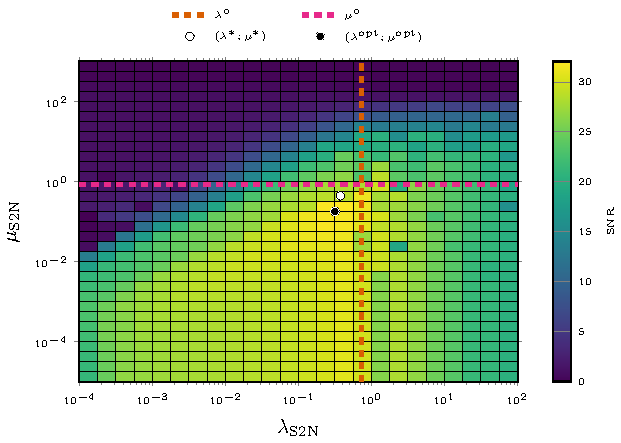
\includegraphics{img/chapitre3/figure5/s2n-hyper.pdf}
    \caption{S2N: SNR en fonction de $(\gls{ls2n},\gls{ms2n})$. Le repère blanc indique la position des paramètres $(\gls{ls2n}^*,\gls{ms2n}^*)$ réglés en suivant la procédure décrite à la section~\ref{sec-s2n-param-tuning}. Les lignes verticale et horizontale correspondent aux valeurs intermédiaires $\gls{ls2n}=\gls{ls2n}^{\circ}$ et $\gls{ms2n}=\gls{ms2n}^\circ$ obtenues au cours de la procédure. Le marqueur noir montre le jeu de paramètre optimal $(\gls{ls2n}^{\mathrm{opt}},\gls{ms2n}^{\mathrm{opt}})$ conduisant au SNR maximal sur la grille.
        \protect\label{fig-s2n-params-tuning}}
\end{figure}

La figure~\ref{fig-s2n-params-tuning} représente les résultats de performances de l'algorithme S2N en fonction des paramètres $(\gls{ls2n},\gls{ms2n})$ sur une grille prédéfinie. En particulier, le SNR maximal obtenu sur la grille est marqué d'un point noir tandis que les valeurs renvoyées par la méthode décrite à la section~\ref{sec-s2n-param-tuning} sont données avec un point blanc. Les lignes verticales et horizontales correspondent aux valeurs intermédiaires $\gls{ls2n}^{\circ}$ et $\gls{ms2n}^\circ$ obtenues au cours du processus en ajustant indépendamment les régularisations spatiale et spectrale tout en supprimant l'autre. 
%
Comme attendu, cette figure montre que le SNR optimal est atteint pour des valeurs non-nulles de chaque paramètre, démontrant ainsi que les deux régularisations spatiale et spectrale sont nécessaires. En effet, des valeurs extrêmes de \gls{ls2n} donnent des images trop lisses ou trop bruitées. De manière similaire, un paramètre \gls{ms2n} trop élevé conduit à une image nulle tandis qu'une valeur trop faible ne régularise pas spectralement l'image. 
%
De plus, les valeurs intermédiaires $\gls{ls2n}^{\circ}$ et $\gls{ms2n}^\circ$ obtenues en ajustant séparément les régularisations tendent à sur-estimer chaque paramètre par rapport à sa valeur optimale. Ce comportement était attendu et modifier l'échelle de ces paramètres comme expliqué à la section~\ref{sec-s2n-param-tuning} conduit à un choix raisonnablement efficace. Notons toutefois que les valeurs estimées ont beau être proches des paramètres optimaux, les valeurs du SNR reportées à la \tabname~\ref{table-s2n-3s-params} montrent que l'ajustement automatique des paramètres conduit à une perte de près de 4dB par rapport à un réglage optimal~: l'algorithme semble être assez sensible aux paramètres.

\begin{table}[b]
    \centering
    \bgroup
    \def\arraystretch{1.7}%
    \begin{tabular}{*{2}{M{3cm}} M{2cm}}
        \toprule
        Paramètres & Valeurs & SNR (dB)\\
        \midrule
        \multirow{ 2}{*}{(\gls{ls2n},\gls{ms2n})}&
        $(\gls{ls2n}^{\mathrm{opt}},\gls{ms2n}^{\mathrm{opt}})$	
        &$32,07$\\
        %
        &$(\gls{ls2n}^*, \gls{ms2n}^*)$
        &$28,18$\\
        %
        \midrule
        \gls{m3s} &
        $1$ &
        $\mathbf{36,03}$\\
        \bottomrule
    \end{tabular}
    \egroup
    \caption{Le SNR associé à S2N et 3S pour des valeurs particulières des paramètres. Les meilleurs scores apparaissent en gras.
        \protect\label{table-s2n-3s-params}}
\end{table}

Grâce à sa formulation contrainte, l'algorithme 3S requiert seulement l'ajustement d'un paramètre de régularisation, à savoir \gls{m3s} qui équilibre la contribution relative des régularisations spatiale et spectrale. Quand \gls{m3s} est trop faible, la régularisation spatiale devient prépondérante, conduisant à une image très lisse. Au contraire, lorsque \gls{m3s} est trop élevé, la régularisation spectrale devient prépondérante, seules les premières lignes de \gls{S} sont non-nulles et l'image n'est pas suffisamment lisse. Des expériences ont montré que 3S n'est pas vraiment sensible au choix du paramètre et que choisir $\gls{m3s}=1$ donne un résultat très satisfaisant (le SNR correspondant est donné à la \tabname~\ref{table-s2n-3s-params}). Cette valeur sera utilisée pour la suite des expériences conduites dans cette section.


\subsection{Impact du niveau de bruit et du taux d'échantillonnage sur les performances}

Les deux algorithmes ont été mis en \oe{}uvre pour différents niveaux de bruit et taux d'échantillonnage $r$. Nous avons moyenné le SNR sur 10 simulations de Monte Carlo, la matrice de bruit \gls{E} étant tirée indépendamment pour chacune d'entre elle tandis que le masque d'échantillonnage \gls{Phi} est resté constant. 
%
Les résultats sont donnés à la figure~\ref{fig-s2n-3s-noise-ratio}.
%
A la vue de cette figure, 3S semble donner de meilleures performances de reconstruction, avec un SNR supérieur et une variance moindre. Au contraire, S2N renvoie un SNR inférieur (presque \np[dB]{10} de moins que 3S) et une variance bien supérieure, spécialement pour de faibles niveaux de bruit.
%
Cette différence entre les deux algorithmes peut s'expliquer de trois manières. D'abord, comme nous l'avons vu précédemment, le paramètre de S2N semble être plus délicat à régler. Ensuite, la norme nucléaire utilisée dans S2N  est connue pour biaiser la solution, conduisant à une diminution des performances de reconstruction. Enfin, la variance très faible de 3S s'explique par le fort débruitage réalisé en ne conservant que les composantes les plus puissantes de l'ACP.

\begin{figure}[h!]
    \centering
    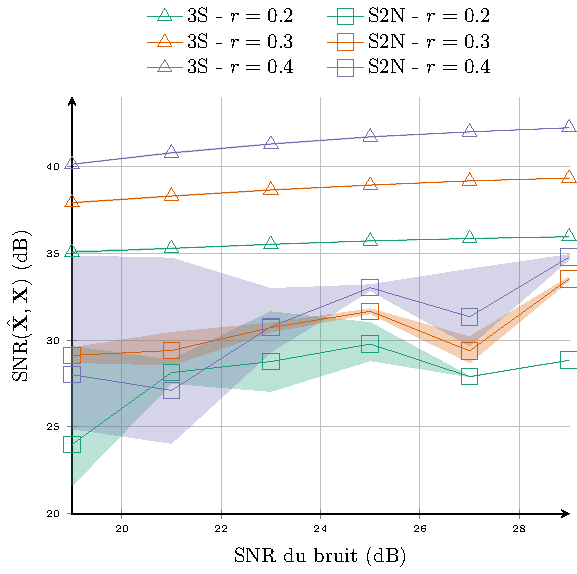
\includegraphics{img/chapitre3/figure6/pix_ratio.pdf}
    \caption{Performances de S2N et 3S en terme de SNR en fonction du taux d'échantillonnage $r$ et du niveau de bruit en SNR. Les régions colorées correspondent aux écart-types. 
        \protect\label{fig-s2n-3s-noise-ratio}}
\end{figure}

\subsection{Comparaison reconstruction / débruitage dans un scénario de démélange}\label{sec-lr-demelange-res}

Des conditions d'acquisition typiques (désigné comme le protocole $\mathcal{P}_0$) sont définies par un échantillonnage séquentiel ($r=1$) avec une durée d'exposition de $\Delta t = \np[ms]{10}$ par pixel. Comme expliqué à la section~\ref{sec-ech-sensibles}, les échantillons biologiques sont facilement détériorés par le faisceau d'électron durant le processus d'acquisition.  Pour résoudre ce problème, la dose totale d'électrons devra être réduite en ajustant soit le taux $r$ de positions visitées, soit le temps $\Delta t$ d'acquisition du spectre à chaque position spatiale.
Deux stratégies d'échantillonnage ont été envisagées afin de réduire les dégâts subis par l'échantillon pour une dose d'électrons donnée.

Le premier protocole, noté $\mathcal{P}_1$, consiste à échantillonner le spectre pour toutes les positions spatiales ($r=1$), mais en réduisant la durée d'acquisition $\Delta t$ pour chaque pixel. La baisse de SNR peut être compensée à l'aide d'une étape de débruitage a posteriori.
%
La seconde stratégie d'acquisition $\mathcal{P}_2$, qui a motivé l'ensemble de ces travaux, consiste à acquérir un sous-ensemble des positions spatiales (\ie{}, $r\leq 1$) avec un temps d'acquisition identique $\Delta t= \np[ms]{10}$ (\ie{}, un SNR supérieur). 
%
Afin de comparer ces deux protocoles d'acquisition, deux jeux de données distincts ont été générés, correspondant à la même énergie de faisceau $\mathcal{E}$
\begin{itemize}
    \item Protocole $\mathcal{P}_1$ : $\Delta t=\np[ms]{2}$, $r=1$,
    \item Protocole $\mathcal{P}_2$ : $\Delta t=\np[ms]{10}$, $r=0,2$.
\end{itemize}
Pour chaque protocole, le niveau de bruit a été ajusté en vue d'atteindre le SNR réaliste rencontré dans une acquisition typique pour un temps d'exposition $\Delta t$ : $\mathrm{SNR} = \np[dB]{19}$ et $\mathrm{SNR} = \np[dB]{25}$ pour les protocoles $\mathcal{P}_1$ et $\mathcal{P}_2$ respectivement.

Pour évaluer l'intérêt du paradigme de l'acquisition partielle, l'exploitabilité de l'image reconstruite après un processus d'acquisition selon le protocole $\mathcal{P}_2$ est comparé avec l'exploitabilité de l'image complète acquise suivant le protocole $\mathcal{P}_1$ en se basant sur l'image vérité terrain générée à la section~\ref{sec-synth-data-lr} (désignée sous le nom d'\emph{oracle} par la suite). De plus, des versions débruitées de l'image acquise suivant le protocole $\mathcal{P}_1$ sont également considérées, où les algorithmes de débruitage sont \gls{acp}+NL-means, S2N et 3S. Ici, \gls{acp}+NL-means consiste à appliquer successivement les deux étapes suivantes : une \gls{acp} tronquée, qui consiste à projeter les données sur le sous-espace défini par les $R_{\mathrm{ACP}}$ composantes principales les plus puissantes (agissant comme une étape de débruitage spectrale) suivi d'une version 3D de NL-means (décrit à la section~\ref{sec-art-patch}) appliquée à l'image débruitée par \gls{acp} (agissant comme une étape de débruitage spatiale et spectrale).
%
La dimension $R_{\mathrm{ACP}}$ a été choisie comme légèrement supérieure à $R$ pour éviter que l'ACP n'enlève de l'information pertinente (en ce qui concerne l'image synthétique où $R_{\mathrm{true}}=3$, $R_{\mathrm{ACP}}$ a été fixé à 10). Notons que des algorithmes de débruitage alternatifs peuvent être considérés, tel que FastHyDe spécialement dédié aux images hyperspectrales~\cite{bioucaspaper}. Par conséquent, 7 spectre-images seront considérés ici:
\begin{itemize}
    \item Oracle : l'image synthétique sans bruit,
    \item les images basées sur un spectre-image complètement acquis suivant le protocole $\mathcal{P}_1$ (désigné comme Full\textsubscript{2ms}) à savoir l'image Full\textsubscript{2ms} et les versions débruitées en utilisant les algorithmes ACP+NL-means, S2N et 3S.
    \item les images basées sur le spectre-image partiellement acquis suivant le protocole $\mathcal{P}_2$ et reconstruit en utilisant S2N et 3S.
\end{itemize}
Ces spectre-images seront désignés par la suite suivant le modèle Protocole-algorithme (\eg{}, $\mathcal{P}_2$-3S est l'image reconstruite en appliquant 3S au spectre-image acquis suivant le protocole $\mathcal{P}_2$).

L'exploitabilité de ces 7 images est évaluée en considérant une tâche conventionnelle fréquemment réalisée en analyse de spectre-image EELS. En effet, puisque les expérimentateurs sont plutôt intéressés par la composition de l'échantillon, ils ont recourt à différentes techniques de démélange introduites à la section~\ref{sec-demelange} en vue de déterminer à la fois les spectres des endmembers et les cartes d'abondance de composants d'intérêt à partir du spectre-image. Par conséquent, pour chaque spectre-image, les spectres élémentaires $(\mathbf{m}_k)_{k=1,\dots,N_c}$ ont été extraits en utilisant l'algorithme SISAL sur les données acquises suivant les protocoles $\mathcal{P}_1$ et $\mathcal{P}_2$. La qualité de la matrice d'endmember estimée $\hat{\mathbf{M}}$ est évaluée en utilisant la métrique $\mathrm{aSAD}(\hat{\mathbf{M}},\mathbf{M})$ définie à l'équation~\eqref{eq-aSAD-def} afin de se protéger de potentiels changements d'échelle.

En se basant sur l'estimation des endmembers, les cartes d'abondance $\mathbf{A}$ sont estimées à partir des images comparées en utilisant l'algorithme SUNSAL. La pertinence des cartes d'abondance estimées est évaluée en calculant le $\mathrm{SNR}(\hat{\mathbf{A}}, \mathbf{A})$ comme défini à l'équation~\eqref{eq-SNR-def}.

En plus de cette évaluation quantitative en terme de performances de démélange, une évaluation qualitative est conduite en inspectant visuellement les spectre-images comparés. Des compositions synthétiques rouge-vert-bleu des images d'intérêt sont générés en sélectionnant 3 niveaux d'énergie spécifiques associés à la présence d'un élément chimique particulier : $b_\mathrm{rouge} = \np[eV]{236}$ (carbone), $b_\mathrm{vert} = \np[eV]{346}$ (calcium) et $b_\mathrm{bleu} = \np[eV]{709}$ (oxygène). Pour s'assurer que les comparaisons entre les images soient justes, les canaux sont indépendamment mis à l'échelle selon une dynamique commune à toutes les images.

\begin{table}[]
    \centering
    \caption{Performances de reconstruction et de démélange. Les meilleurs scores apparaissent en gras.
        \protect\label{tab-lr-metrics}}
    \bgroup
    \def\arraystretch{1.5}%
    \begin{tabular}{*{5}{M{1.6cm}}}
        \toprule
        Protocole & Algorithme
        &$\mathrm{SNR}$ $(\hat{\mathbf{X}}, \mathbf{X})$        
        &$\mathrm{aSAD}$ $(\hat{\mathbf{M}}, \mathbf{M})$    
        &$\mathrm{SNR}$ $(\hat{\mathbf{A}}, \mathbf{A})$\\
        \midrule
        %
\multicolumn{2}{c}{Oracle}     & $\infty$                & 0,07014        & 6,631 \\%
\midrule
\multirow{4}*{$\mathcal{P}_1$} & Full\textsubscript{2ms} & 19,22          & 0,14321          & 3,330 \\%
                               & ACP+NL-means            & 42,92          & 0,14321          & 3,382 \\%
                               & S2N                     & 33,33          & 0,14321          & 3,481 \\%
                               & 3S                      & \textbf{43,28} & 0,14321          & 3,253 \\%
\midrule
\multirow{2}*{$\mathcal{P}_2$} & S2N                     & 30,00          & \textbf{0,11025} & 3,375 \\%
                               & 3S                      & 35,90          & \textbf{0,11025} & \textbf{4,304} \\
        %
        \bottomrule
        %
    \end{tabular}
\egroup
\end{table}

\begin{mylandscape}
    \begin{normalfigure}
        \centering
        \newlength\figurelength
\setlength\figurelength{2.3cm}

\bgroup
    \def\arraystretch{1.5}%
    \begin{tabular}{M{0.02cm}*{8}{M{2.5cm}}}
        %
        &&Oracle&
        $\mathcal{P}_1$-Full\textsubscript{2ms}&
        $\mathcal{P}_1$-ACP+NL-means&
        $\mathcal{P}_1$-S2N &
        $\mathcal{P}_1$-3S&
        $\mathcal{P}_2$-S2N&
        $\mathcal{P}_2$-3S\\
        %
        %\rotatebox{90}{Spim}
        \multicolumn{2}{M{1.8cm}}{Vraies cartes d'abondance}
        &
\includegraphics[width=\figurelength]{img/chapitre3/figure7/img2_1.png}
        &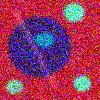
\includegraphics[width=\figurelength]{img/chapitre3/figure7/img2_2.png}
        &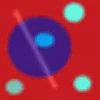
\includegraphics[width=\figurelength]{img/chapitre3/figure7/img2_3.png}
        &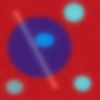
\includegraphics[width=\figurelength]{img/chapitre3/figure7/img2_5.png}
        &
\includegraphics[width=\figurelength]{img/chapitre3/figure7/img2_6.png}
        &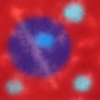
\includegraphics[width=\figurelength]{img/chapitre3/figure7/img2_7.png}
        &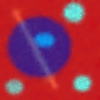
\includegraphics[width=\figurelength]{img/chapitre3/figure7/img2_8.png}\\
        %
        \rotatebox{90}{Résine}
        &
\includegraphics[width=\figurelength]{img/chapitre3/figure7/maps/img_1_1.png}
        &
\includegraphics[width=\figurelength]{img/chapitre3/figure7/maps/img_2_1.png}
        &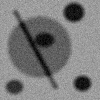
\includegraphics[width=\figurelength]{img/chapitre3/figure7/maps/img_3_1.png}
        &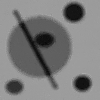
\includegraphics[width=\figurelength]{img/chapitre3/figure7/maps/img_4_1.png}
        &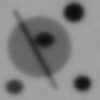
\includegraphics[width=\figurelength]{img/chapitre3/figure7/maps/img_6_1.png}
        &
\includegraphics[width=\figurelength]{img/chapitre3/figure7/maps/img_7_1.png}
        &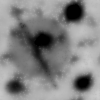
\includegraphics[width=\figurelength]{img/chapitre3/figure7/maps/img_8_1.png}
        &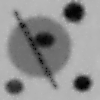
\includegraphics[width=\figurelength]{img/chapitre3/figure7/maps/img_9_1.png}\\
        %
        \rotatebox{90}{Organique 1}
        &
\includegraphics[width=\figurelength]{img/chapitre3/figure7/maps/img_1_2.png}
        &
\includegraphics[width=\figurelength]{img/chapitre3/figure7/maps/img_2_2.png}
        &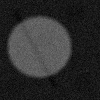
\includegraphics[width=\figurelength]{img/chapitre3/figure7/maps/img_3_2.png}
        &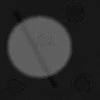
\includegraphics[width=\figurelength]{img/chapitre3/figure7/maps/img_4_2.png}
        &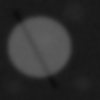
\includegraphics[width=\figurelength]{img/chapitre3/figure7/maps/img_6_2.png}
        &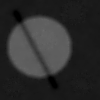
\includegraphics[width=\figurelength]{img/chapitre3/figure7/maps/img_7_2.png}
        &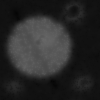
\includegraphics[width=\figurelength]{img/chapitre3/figure7/maps/img_8_2.png}
        &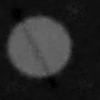
\includegraphics[width=\figurelength]{img/chapitre3/figure7/maps/img_9_2.png}\\
        %
        \rotatebox{90}{Organique 2}
        &
\includegraphics[width=\figurelength]{img/chapitre3/figure7/maps/img_1_3.png}
        &
\includegraphics[width=\figurelength]{img/chapitre3/figure7/maps/img_2_3.png}
        &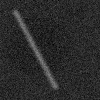
\includegraphics[width=\figurelength]{img/chapitre3/figure7/maps/img_3_3.png}
        &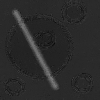
\includegraphics[width=\figurelength]{img/chapitre3/figure7/maps/img_4_3.png}
        &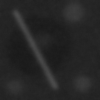
\includegraphics[width=\figurelength]{img/chapitre3/figure7/maps/img_6_3.png}
        &
\includegraphics[width=\figurelength]{img/chapitre3/figure7/maps/img_7_3.png}
        &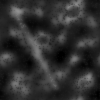
\includegraphics[width=\figurelength]{img/chapitre3/figure7/maps/img_8_3.png}
        &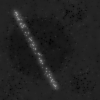
\includegraphics[width=\figurelength]{img/chapitre3/figure7/maps/img_9_3.png}\\
        %
        \rotatebox{90}{Calcification}
        &
\includegraphics[width=\figurelength]{img/chapitre3/figure7/maps/img_1_4.png}
        &
\includegraphics[width=\figurelength]{img/chapitre3/figure7/maps/img_2_4.png}
        &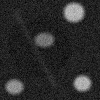
\includegraphics[width=\figurelength]{img/chapitre3/figure7/maps/img_3_4.png}
        &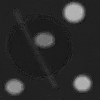
\includegraphics[width=\figurelength]{img/chapitre3/figure7/maps/img_4_4.png}
        &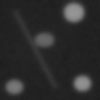
\includegraphics[width=\figurelength]{img/chapitre3/figure7/maps/img_6_4.png}
        &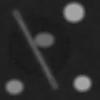
\includegraphics[width=\figurelength]{img/chapitre3/figure7/maps/img_7_4.png}
        &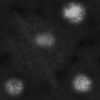
\includegraphics[width=\figurelength]{img/chapitre3/figure7/maps/img_8_4.png}
        &\includegraphics[width=\figurelength]{img/chapitre3/figure7/maps/img_9_4.png}\\
    \end{tabular}
\egroup
        \caption{Ligne 1 : composition colorée des spectres-images oracle, acquis (Full\textsubscript{2ms}), débruités (protocole $\mathcal{P}_1$) et reconstruits (protocole $\mathcal{P}_2$). Lignes 2-5 : les cartes d'abondance estimées par SUNSAL pour les spectre-images correspondants.% \the\textwidth
            \protect\label{fig-lr-maps}}
    \end{normalfigure}
\end{mylandscape}

Les résultats quantitatifs sont reportés à la \tabname~\ref{tab-lr-metrics} tandis que les images reconstruites et les cartes d'abondance estimées sont représentées à la figure~\ref{fig-lr-maps}. Notons que les résultats de démélange obtenus des six images acquises, débruitées et reconstruites, sont aussi comparés à ceux obtenus directement sur l'image vérité terrain \gls{X}. Ces estimations oracle donnent les performances les plus optimistes pouvant être atteintes en démélangeant les images débruitées ou reconstruites. Notons également que le SNR associé à l'oracle est infini puisque l'image oracle est exactement la vérité terrain \gls{X}, tandis que la $\mathrm{aSAD}(\hat{\mathbf{M}}, \mathbf{M})$ est non-nul et le $\mathrm{SNR}(\hat{\mathbf{A}}, \mathbf{A})$ n'est pas infini puisque les algorithmes de démélange ne permettent pas de retrouver exactement les endmembers et les cartes d'abondance utilisées pour générer \gls{X}. Notons enfin que la $\mathrm{aSAD}(\hat{\mathbf{M}}, \mathbf{M})$ est constante pour toutes les méthodes au sein d'un protocole puisque SISAL est appliqué aux données acquises.

Nous pouvons d'abord observer que débruiter l'image acquise suivant le protocole $\mathcal{P}_1$ conduit à un SNR significativement supérieur pour les spectres-images par rapport à ceux obtenus en reconstruisant l'image acquise suivant le protocole $\mathcal{P}_2$ (mis à part $\mathcal{P}_1$-S2N qui donne des résultats moins bons que $\mathcal{P}_2$-3S). Les algorithmes de reconstruction proposés couplés à l'acquisition partielle semblent être moins performants, bien que le SNR est supérieur pendant le processus d'acquisition. Toutefois, les performances concernant la tâche de démélange sont en faveur du protocole $\mathcal{P}_2$. En effet, les spectres élémentaires sont mieux restitués chez les images acquises avec une durée d'exposition plus grande que chez les images acquises avec une durée d'exposition plus courte, même après une étape de débruitage. Ces résultats étaient assez attendus pour les spectres estimés des endmembers, puisque les pixels observés dans le cadre de l'échantillonnage partiel ont un SNR plus grand. Ainsi, l'algorithme d'extraction d'endmember SISAL peut exploiter des spectres plus fiables afin d'estimer les signatures des matériaux élémentaires. De plus, les cartes d'abondances estimées à partir de l'image reconstruite par l'algorithme proposé 3S permettent d'atteindre un SNR supérieur, prouvant que cette image reconstruite peut être exploitée avec confiance pour cartographier les éléments du spectre-image.

De manière qualitative, une inspection visuelle des cartes d'abondance représentées à la figure~\ref{fig-lr-maps} montre que les techniques S2N et 3S produisent des images plus rugueuses, avec quelques trous correspondant aux régions non échantillonnées. Mais il y a moins de mélange entre les différents éléments, par exemple, les cartes de organique 1 et organique 2 sont particulièrement bien dissociées pour l'image reconstruite par 3S. Pour résumer, pour une dose d'électrons identique, l'échantillonnage partiel semble permettre une meilleure extraction des endmembers et une meilleure restitution de détails du spectre que le débruitage, même si des structures spatiales fines (comme organique 2 dans notre exemple) pourraient être cartographiées avec moins de précision.

Finalement, nous pouvons observer qu'utiliser les algorithmes 3S et S2N comme procédure de débruitage donne des erreurs comparables à ACP+NL-means (sauf pour le SNR de $\mathcal{P}_1$-S2N). Cependant, les résultats de démélange de $\mathcal{P}_1$-3S sont significativement moins bons que $\mathcal{P}_1$-ACP+NLmeans. 



%
\section{Résultats sur des données réelles}\label{sec-3s-real-data}

Dans cette section, les techniques de reconstruction proposées sont appliquées à un échantillon réel\footnote{Il s'agit de l'échantillon dont ont été extraits les spectres \gls{Mu} ayant servi à générer les données synthétiques à la section~\ref{sec-synth-data-lr}.} dont l'image HAADF en niveau de gris est donné à la figure~\ref{fig-BR-haadf-a} et dont quelques représentations spectrales sont données à la figure~\ref{fig-lr-real-data-spectra}. 
%
Cet échantillon est un tissu biologique analysé dans~\cite{gay2020nanoscale} contenant des particules faites de phosphate de calcium. L'échantillon a été chimiquement fixé, déshydraté et incrusté dans une résine époxy. Les éléments analysés sont listés dans la section~\ref{sec-synth-data-lr}, à savoir le carbone, le calcium, l'azote et l'oxygène. Cet échantillon a été acquis à l'aide du microscope STEM VG HB 501 équipé d'un système d'échantillonnage partiel.

\begin{normalfigure*}
    \centering
    \subfigure[\protect\label{fig-lr-real-data-spectra-a}Position des pixels et des zones représentées]{
        \includegraphics[width=0.3\textwidth]{img/chapitre3/figure12/loc-image-bis.png}}\\
    \subfigure[\protect\label{fig-lr-real-data-spectra-b}Spectres centraux]{
        \includegraphics[width=0.7\textwidth]{img/chapitre3/figure12/spectra-center.pdf}}\\
    \subfigure[\protect\label{fig-lr-real-data-spectra-c}Spectres moyennés]{
        \includegraphics[width=0.7\textwidth]{img/chapitre3/figure12/spectra-mean.pdf}}\\
    \caption{\protect\label{fig-lr-real-data-spectra}
        Représentations spectrales de l'échantillon réel étudié acquis suivant le protocole $\mathcal{P}_0$ ($\Delta t=\np[ms]{10}$, $r = 1$).
        \subref{fig-lr-real-data-spectra-a}~Image HAADF de l'échantillon où trois zones distinctes sont représentées. Les pixels centraux de ces zones sont également mis en évidence.
        \subref{fig-lr-real-data-spectra-b}~Représentation des trois spectres associés aux pixels centraux.
        \subref{fig-lr-real-data-spectra-c}~Représentation de la moyenne des spectres pour chaque zone.
    }
\end{normalfigure*}

Dans les conditions expérimentales, trois protocoles distincts sont considérés pour acquérir l'échantillon :
\begin{itemize}
    \item Protocole $\mathcal{P}_0$ : $\Delta t=\np[ms]{10}$, $r = 1$,
    \item Protocole $\mathcal{P}_1$ : $\Delta t=\np[ms]{2}$, $r = 1$,
    \item Protocole $\mathcal{P}_2$ : $\Delta t=\np[ms]{10}$, $r = 0,2$.
\end{itemize}
Le protocole $\mathcal{P}_0$ correspond à des paramètres d'acquisition usuels pour ce type d'échantillon. Les spectre-images associés aux protocoles $\mathcal{P}_0$ à $\mathcal{P}_2$ sont respectivement appelés Full\textsubscript{2ms}, Full\textsubscript{10ms} et Partiel. En poursuivant la notation Protocole-Algorithme introduite dans la section précédente, les spectre-images comparés ici sont
\begin{itemize}
    \item les images entièrement échantillonnées $\mathcal{P}_0$-Full\textsubscript{10ms} et $\mathcal{P}_1$-Full\textsubscript{2ms},
    \item l'image débruitée $\mathcal{P}_1$-ACP+NL-means,
   \item  les images reconstruites $\mathcal{P}_2$-S2N et $\mathcal{P}_2$-3S.
\end{itemize}
Les images acquises sont de taille $51\times 51$ et des compositions colorées synthétiques de ces images sont représentées à la figure~\ref{fig-lr-real-spims} où $\mathcal{P}_1$-Full\textsubscript{2ms} est utilisé comme référence pour définir la dynamique commune. Concernant les paramètres de S2N et de 3S, le paramètre de régularisation de S2N à été choisi en effectuant la procédure décrite à la section~\ref{sec-s2n-param-tuning} tandis que le paramètre \gls{m3s} de 3S a été affiné à la main afin d'obtenir un compromis entre les régularisations spatiale et spectrale.

\begin{normalfigure*}[] 
    \centering
    %
    \subfigure[$\mathcal{P}_0$-Full\textsubscript{10ms}]{
        \includegraphics[width=0.20\textwidth]{img/chapitre3/figure9/2-X10ms.png} }\hspace{0.3cm}
    \subfigure[$\mathcal{P}_1$-Full\textsubscript{2ms}]{
        \includegraphics[width=0.20\textwidth]{img/chapitre3/figure9/1-X2ms.png} }\hspace{0.3cm}
    \subfigure[$\mathcal{P}_2$-Partial]{
        \includegraphics[width=0.20\textwidth]{img/chapitre3/figure9/5-NoisyPart.png} }\\
    %
    \subfigure[$\mathcal{P}_1$-ACP+NL-means]{
        \includegraphics[width=0.20\textwidth]{img/chapitre3/figure9/4-X2msDe.png} }\hspace{0.3cm}
    \subfigure[$\mathcal{P}_2$-S2N]{
        \includegraphics[width=0.20\textwidth]{img/chapitre3/figure9/6-SNN.png} }\hspace{0.3cm}
    \subfigure[$\mathcal{P}_2$-3S]{
        \includegraphics[width=0.20\textwidth]{img/chapitre3/figure9/3-SSS.png} }
    %
    \caption{Compositions colorées des spectre-images réels.\protect\label{fig-lr-real-spims}}
\end{normalfigure*}

Comme à la section précédente, en vue d'évaluer les performances des méthodes proposées, les images sont démélangées en utilisant SISAL pour extraire les signatures des matériaux et SUNSAL pour estimer les cartes d'abondance correspondantes. Les cartes sont données à la figure~\ref{fig-lr-maps-real} tandis que les signatures des endmembers sont données à la figure~\ref{fig-lr-spectra-real}. Un nombre de $N_c=5$ composantes a été choisi, mais seules les trois plus significatives sont affichées. 

%
\begin{normalfigure*}[hbtp]
    \centering
    \bgroup
\def\arraystretch{1.5}%
\begin{tabular}{M{0.02cm}*{5}{M{2.4cm}}}
%
&
$\mathcal{P}_0$-Full\textsubscript{10ms}&
$\mathcal{P}_1$-Full\textsubscript{2ms}&
$\mathcal{P}_1$-ACP+NL-means&
$\mathcal{P}_2$-S2N&
$\mathcal{P}_2$-3S\\
%
\rotatebox{90}{Carte \#1}&
\includegraphics[width=2.3cm]{img/chapitre3/figure10/1-Full10ms_1.png}&
\includegraphics[width=2.3cm]{img/chapitre3/figure10/2-Full2ms_1.png}&
\includegraphics[width=2.3cm]{img/chapitre3/figure10/3-PCA+NLm_1.png}&
\includegraphics[width=2.3cm]{img/chapitre3/figure10/7-P2-S2N_1.png}&
\includegraphics[width=2.3cm]{img/chapitre3/figure10/8-P2-3S_1.png}\\
%
\rotatebox{90}{Carte \#2}&
\includegraphics[width=2.3cm]{img/chapitre3/figure10/1-Full10ms_2.png}&
\includegraphics[width=2.3cm]{img/chapitre3/figure10/2-Full2ms_2.png}&
\includegraphics[width=2.3cm]{img/chapitre3/figure10/3-PCA+NLm_2.png}&
\includegraphics[width=2.3cm]{img/chapitre3/figure10/7-P2-S2N_2.png}&
\includegraphics[width=2.3cm]{img/chapitre3/figure10/8-P2-3S_2.png}\\
%
\rotatebox{90}{Carte \#3}&
\includegraphics[width=2.3cm]{img/chapitre3/figure10/1-Full10ms_3.png}&
\includegraphics[width=2.3cm]{img/chapitre3/figure10/2-Full2ms_3.png}&
\includegraphics[width=2.3cm]{img/chapitre3/figure10/3-PCA+NLm_3.png}&
\includegraphics[width=2.3cm]{img/chapitre3/figure10/7-P2-S2N_3.png}&
\includegraphics[width=2.3cm]{img/chapitre3/figure10/8-P2-3S_3.png}\\
%
\end{tabular}
\egroup
    \caption{Cartes d'abondance estimées avec SUNSAL.\protect\label{fig-lr-maps-real}}
\end{normalfigure*}
%
\begin{mylandscape}
    \begin{normalfigure}
        \centering
        \includegraphics[]{img/chapitre3/figure11/template.pdf}\\
        \includegraphics[]{img/chapitre3/figure11/spectrum-2-zoom.pdf}
        \caption{Lignes 1 à 3 : trois spectres élémentaires (sur cinq) estimés par SISAL après démélange. Ligne 4 : zoom sur les seuils Ca $L_{2, 3}$ du spectre 2 (mis en évidence à la ligne 2). Les amplitude sont en fonction de la perte d'énergie (en eV).\protect\label{fig-lr-spectra-real}}
    \end{normalfigure}
\end{mylandscape}

Visuellement parlant, faire l'acquisition suivant le protocole $\mathcal{P}_1$ puis débruiter semble donner les meilleurs résultats puisque les spectre-images comme les cartes d'abondance montrent une meilleure résolution spatiale, permettant de révéler plus de détails dans la carte numéro 2 associée aux calcifications, par exemple. 
%
Au contraire, les schémas basés sur l'échantillonnage partiel révèlent des pics de grande intensité dans le spectre-image et dans les cartes d'abondances associées, ce qui réduit la résolution spatiale.
%
Remarquons que les spectre-images complets acquis suivant les protocoles $\mathcal{P}_0$ et $\mathcal{P}_1$ sont déjà sous-échantillonnés en vue de préserver l'échantillon, comme discuté à la section~\ref{sec-donnees-sous-echantillonnees}, et leur résolution est faible. Par conséquent, le spectre-image acquis suivant le protocole $\mathcal{P}_2$ est \emph{fortement} sous-échantillonné, ce qui détériore particulièrement les performances spatiales, comme nous l'avons vu.

Toutefois, les caractéristiques spectrales sont mieux restituées sous acquisition partielle avec $\Delta t=\np[ms]{10}$ (\ie\ sous le protocole $\mathcal{P}_2$) et avec 3S comme algorithme de reconstruction. En effet, la séparation des seuils Ca $L_{2, 3}$ est clairement visible sur le spectre numéro 2 extrait des spectre-images reconstruits après le protocole $\mathcal{P}_2$ (voir la ligne 4 dans la figure~\ref{fig-lr-spectra-real}). Ces seuils sont également visibles pour le second spectre de $\mathcal{P}_2$-S2N, mais le troisième spectre donne des résultats insatisfaisants, pouvant venir d'un mauvais choix de paramètres ou du biais introduit par la norme nucléaire. Toutefois, cette séparation $L_{2, 3}$ n'est pas visible pour le 2\textsuperscript{ième} spectre extrait des images débruitées après le protocole $\mathcal{P}_1$. Cependant, il faut noter dans ce cas que le faible nombre de pixels ($51\times 51$) comparé aux données synthétiques générée à la section~\ref{sec-lr-demelange-res} ($100\times 100$) rend l'extraction de composantes par SISAL moins performante. 
%
Ainsi, le choix de la stratégie d'acquisition doit résulter d'un compromis entre les résolutions spectrales et spatiales requises. 
%
 


%
\section{Conclusion}

Dans ce chapitre, nous avons introduit de nouvelles techniques de reconstruction afin de préserver l'échantillon dans le cadre de l'acquisition partielle de spectre-images EELS basse résolution. Elles se basent sur des connaissances a priori des spectre-images spatialement lisses, à savoir la régularité spatiale et le faible rang spectral. 
%
Deux algorithmes ont été proposés pour réaliser l'étape de reconstruction et des expériences ont comparé cette approche avec un schéma d'acquisition standard. Les résultats ont montré que l'algorithme 3S est plus performant que S2N aussi bien en termes de qualité de reconstruction que de temps d'exécution.

En comparant avec une acquisition standard (complète) suivie d'une opération de débruitage, le schéma d'acquisition partielle couplé avec la méthode 3S a permis une meilleure estimation spectrale, tandis que certains détails spatiaux semblaient détériorés. 
%
La cause principale de cette détérioration semble être que le spectre-image, même complètement acquis, peut initialement être de résolution très faible afin de préserver l'échantillon. Par conséquent, l'acquisition partielle du spectre-image dégrade encore davantage les informations spatiales disponibles. Pour corriger ce problème, les techniques de reconstruction proposées pourraient être couplées à de la super-résolution, restituant ainsi la résolution autorisée par le microscope.

